\chapter{Kontextabgrenzung}
\label{ch:Kontextabgrenzung}
In der Kontextabgrenzung grenzen wir alle Kommunikationspartner vom System ab und stellen somit unsere externen Schnittstellen fest. Dazu wird der Kontext einerseits fachlich, als auch technisch voneinander abgegrenzt.
\section{Fachlicher Kontext}
Die fachliche Kontextabgrenzung dient uns dazu alle Kommunikationspartner zusammen mit den jeweiligen Ein- und Ausgabedaten mit dem System zu erläutern. Folgende Abbildung veranschaulicht die fachliche Kontextabgrenzung:
\begin{figure}[h]
	\centering
	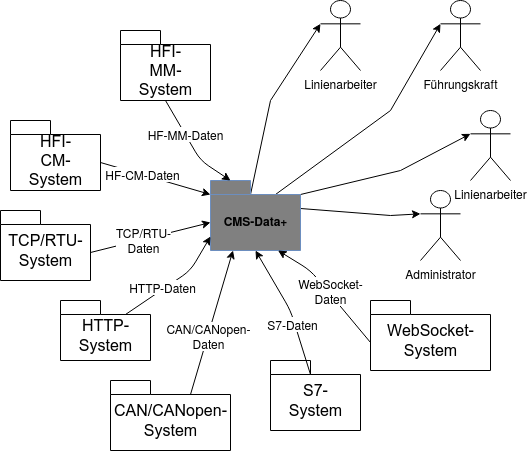
\includegraphics[width=0.6\textwidth]{Graphics/fachliche_kontextabgrenzung.png}
	\caption{Fachliche Kontextabgrenzung}
	\label{fig:fachliche_kontextabgrenzung}
\end{figure}

Wie das Diagramm veranschaulicht, dient das Data+ als Datensenke für alle angezeigten Systeme. Jedes dieser Systeme kann über eine eigene Schnittstelle bzw. Protokoll verfügen und darüber die protokollspezifischen Daten an das Data+ System senden.
Folgende Tabelle stellt noch einmal die Kommunikationspartner und den fachlichen Kontext zum System dar.\\↔
\begin{table}[th]
	\begin{tabularx}{\textwidth}{|p{3.5cm}|p{7cm}|X|}
		\hline
		Kommunikations-
		partner & Beschreibung & Technologie \\
		\hline
		HFI-MM-Feldgerät &Feldgerät schickt während der Betriebszeit seine Sensordaten an CMS  & HFI-MM-Protokolldaten über Bussystem\\
		\hline
		HFI-CM-Feldgerät & Feldgerät schickt während der Betriebszeit seine Sensordaten an CMS  & HFI-CM-Protokolldaten über Bussystem\\
		\hline
		TCP/RTU-Feldgerät &Feldgerät schickt während der Betriebszeit seine Sensordaten an CMS  & Modubus TCP/RTU Protokolldaten über Bussystem \\
		\hline
		HTTP-System & 4 verschiedene Arten von Daten (User, Group, Station, Datapoint) von dem CMS aus lesen und schreiben zu können & Daten nach JSON-Schema-Format \\
		\hline
		CAN/CANopen-Feldgerät & Feldgerät schickt während der Betriebszeit seine Sensordaten an CMS senden & CAN/CANopen-Protokolldaten nach Standard\\
		\hline
		S7-Feldgerät &Feldgerät schickt während der Betriebszeit seine Sensordaten an CMS senden & S7-Protokolldaten nach Standard\\
		\hline
		OPC-UA-Server & Wenn ein Server im CMS registriert ist, sollen dessen Daten an das CMS weiterleitet werden & Daten nach Schemadefinition\\
		\hline
		OPC-UA-Client & Wird ein Client im CMS registriert, so sollen Daten an ihn weitergeleitet werden & Daten nach Schemadefinition\\
		\hline
		Linienarbeiter & Sollen während der Betriebszeit die Daten ihrer aktuellen Maschine gesendet bekommen & Webbrowser\\
		\hline
		Führungskraft & Nach der Betriebszeit aufbereitete Daten über den Tagesverlauf und möglichen Zustand der Maschine & Webbrowser\\
		\hline
		Entwickler & Empfängt zur beliebigen Zeit, unaufbereitete Daten & Hexadezimal/JSON-Format über Konsole oder Weboberfläche\\
		\hline
		Administrator & Während der Betriebszeit sollen Fehlerreports an den Administrator gesendet werden & Webbrowser\\
		\hline
	\end{tabularx} 
	\caption{Fachliche Kontextabgrenzung der Kommunikationspartner}
	\label{tab:FachlicheKontextabgrenzungDerKommunikationspartner}
\end{table}
Alle einzelnen Kommunikationspartner haben selbst wiederum Eingangsdaten und geben alle Daten aus verschiedenen Protokollen dem System under Design (SUD) weiter. Dieses verarbeitet die eingehenden Daten und wertet diese aus.
\clearpage
\section{Technischer Kontext}
Der technische Kontext definiert die Kanäle und das Übertragungsmedium über dem unser System mit externen Komponenten interagiert. Dabei wird erklärt, wie und über welche technischen Kanäle unsere fachlichen Ein- und Ausgaben ablaufen. Zur Veranschaulichung wird dies im folgenden Diagramm dargestellt:

\begin{figure}[h]
	\centering
	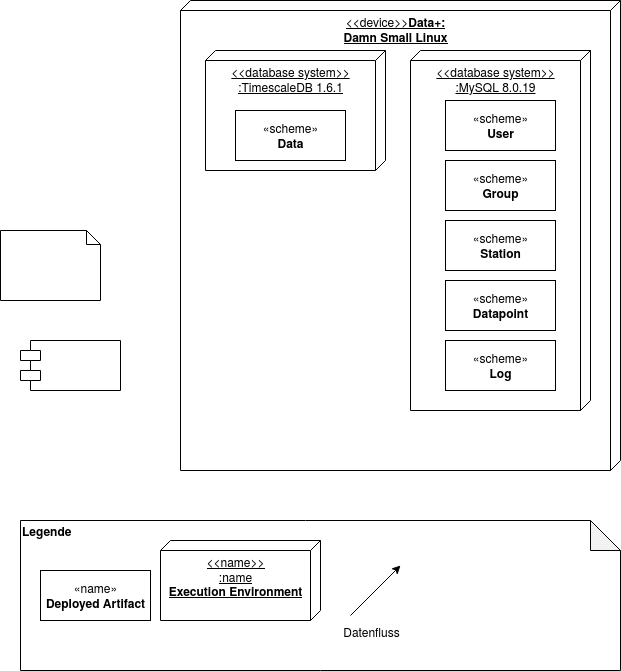
\includegraphics[width=1\textwidth]{Graphics/technische_kontextabgrenzung.png}
	\caption{Technische Kontextabgrenzung}
	\label{fig:technische_kontextabgrenzung}
\end{figure}
Das Gesamtsystem wird auf einem embedded Device mit Linux als Betriebssystem laufen. Dazu soll das Gerät reine Rohdaten von den aufgelisteten Systemen aufnehmen können. Die Fremdsysteme und das Device müssen dazu in einem Netzwerk miteinander verbunden sein. Daneben ist es möglich mit einem Webserver, also Technologie basierend auf HTTP und HTTPS, konfigurierende Daten auf das Gerät zu senden. Im Gegenzug kann auch das Gerät alle seine Datentypen den externen Komponenten bekannt machen. Die Hauptfunktion jedoch ist es den Client-Computer mit aufbereiteten Daten über eine Weboberfläche zu versorgen. Währenddessen wird der Deviceeigene Zustand überwacht und ebenso gespeichert.
\begin{table}[t]
	\begin{tabularx}{\textwidth}{|l|X|}
		\hline
		Eingangsdaten & Beschreibung\\
		\hline
		Daten & Dieses Schema, dient dazu jegliche Daten aus den Datenquellen zu speichern. Es enthält folgende Eigenschaften: der Endpunkt von dem die Daten stammen, bestehend aus IP, Port und gegebenenfalls möglicher Adresse, einem Zeitstempel, wann die Daten das Gerät erreicht haben, sowie den Wert der Daten.\\
		\hline
		Datenpunkt & Ein Datenpunkt enthält zusätzliche Informationen zu einem Parameter des Daten-Schemas. So ist in einem Datenpunkt-Datensatz ein Name, zur Beschreibung der Daten zwingend erforderlich. Zusätzlich muss der Typ der korrespondierenden Daten angegeben werden. Dieser kann entweder von Typ Integer-32Bit, String, JSON-Object, Boolean oder Float-32Bit sein. Des Weiteren kann ein Datapoint eine SI-Einheit besitzen. Ein Kontext zu dem Data-Schema, wird aber erst in dem Stations-Schema hergestellt.\\
		\hline
		Station & Ein Stations-Datensatz umfasst einen oder mehrere Datenpunkte und enthält demnach eine Liste von DatenpunktIds. Jedem dieser DatenpunktIds ist eine DatenId zugeordnet, sodass die Werte weiter interpretierbar sind.\\
		\hline
		Benutzer & Dieser Datensatz beschreibt einen Nutzer des Systems. Er enthält die folgenden Eigenschaften: es werden der Vorname, der Nachname, die Personalnummer, ein Benutzername, das Password als Hash-Wert, sowie die Telefonnummer und E-Mailadresse abgespeichert.\\
		\hline
		Gruppe & Die Gruppe dient zur Zusammenfassung mehrerer User, welche die gleichen Rechte für eine Station haben sollen. Dazu enthält jeder Datensatz einen Gruppennamen, die Rollen-Ids, die  StationIds und die BenutzerIds.\\
		\hline
		Rollen & Das Rollen-Schema weist Rechte wie das Lesen, Schreiben und Administrieren von Stationen, Gruppen und Usern zu.\\
		\hline
		Log & In den Log werden Datensätze, die einen Fehlerzustand mit Zeitpunkt und Beschreibung besitzen, geschrieben. Dies können beispielsweise mögliche I/O-Exceptions sein.\\
		\hline
	\end{tabularx} 
	\caption{technische Kontextabgrenzung Daten}
	\label{tab:technischeKontextabgrenzungDaten}
\end{table}
